\renewcommand{\encodingdefault}{OT1}
\documentclass[10pt,conference]{IEEEtran}
\IEEEoverridecommandlockouts
% The preceding line is only needed to identify funding in the first footnote. If that is unneeded, please comment it out.
\usepackage{cite}
\usepackage{amsmath,amssymb,amsfonts}
\usepackage{algorithmic}
\usepackage{graphicx}
\usepackage{textcomp}
\usepackage{xcolor}
\usepackage{underscore}
\usepackage{hyperref}
\usepackage{minted}
\def\BibTeX{{\rm B\kern-.05em{\sc i\kern-.025em b}\kern-.08em
    T\kern-.1667em\lower.7ex\hbox{E}\kern-.125emX}}
\begin{document}

\title{Jitsi on OpenBSD\\
{\Large Puffy presents video conferencing}
}

\author{\IEEEauthorblockN{Philipp Buehler}
\IEEEauthorblockA{
\textit{sysfive.com GmbH}\\
Hamburg, Germany \\
pb-openbsd@sysfive.com}

}

\maketitle

\begin{abstract}
This paper will cover all bits and bolts to fully understand the components
at play, their intercommunications and how this knowledge can be used to create
a Jitsi-on-OpenBSD setup that features a restricted (compartmentalized) setup using
dedicated machines or -as shown- VMM based VMs, where each VM runs only one of the
components.

It'll be documented what's necessary to create a sensible pf.conf on the host, on each VM
and how to add system and application specific startup parameters and configuration of
each component.


\end{abstract}

\begin{IEEEkeywords}
Jitsi, OpenBSD, VMM
\end{IEEEkeywords}

\section{Introduction}
Jitsi and OpenBSD are both not covered much as a documented setup. Installation documents
for Jitsi are almost always about Linux OS (and there mostly Debian) and do not cover
some internals. The reference documentation on the other hand can be very overwhelming.

There is some FreeBSD ``all in one'' port (package) with no explanation and it cannot be
used to install only core components on different nodes.

This documentation is to show a distributed install on OpenBSD nodes using newly developed
native packages and need-to-function (minimum) firewall settings (`pf.conf`).

The described configurations will enable a fully integrated video conferencing
to be available at `https://jts.fips.de` - adapt the shown settings accordingly for your domain.

\section{Riddles}
Both major players show obstacles that have to be overcome to gain a functioning installation.

\subsection{Jitsi}
A "full blown" Jitsi installation can consist of over over a dozen components and the
necessary networking/firewalling configuration can be exhaustive. Any possible discovery
magic is not there but the documentation and examples could lead to suspect that.

Some configuration snippets are undocumented and tend to make the understanding poorer
not better. Worst example are necessary DNS settings, startup variable names and `nginx.conf`.

The typical answer to be found when asking questions is to use the official `all-in-one`
Debian VM or now `docker``.

\subsection{OpenBSD}
This also leds to the question if it's possible to run a (core) Jitsi installation on
OpenBSD only or if there's (technical) need be for Linux.

Also it's a bit difficult to find example-based documentation on VMM, e.g. for using
VMM to provide the VMs and act as the core router, too (`vm.conf`). The networking needed
has to be adapted in `pf.conf`.

Can we scale the installation horizontally and how to use Java based applications
with `rcctl`?

\section{Components}
\subsection{OpenBSD}
In this example setup I make heavy use of `VMM` eco system on OpenBSD which consists of:
\begin{description}
\item[vmm(4) - virtual machine monitor] \hfill \\
	kernel driver isolating/providing the required resources for the VMs (`hypervisor`)
\item[vmd(8)] \hfill \\
	userland daemon to interact with `vmm`
\item[vmctl(8)]  \hfill \\
	administrative tool to create, start/stop, .. VMs
\item[vm.conf(5)]  \hfill \\
	persist VMs resource configuration
\end{description}

\subsection{Jitsi}
A core (basic video conferencing) setup comprised by:
\begin{description}
\item[nginx(8) web] \hfill \\
	serving web assets and reverse proxy BOSH or websockets
\item[prosody(8) xmpp] \hfill \\
	conference chat + internal components communication (esp. “PubSub” for health/discovery)
\item[jicofo - JItsi COnference FOcus] \hfill \\
	room+session handling in conferences (who’s talking to whom and where)
\item[jvb - Jitsi videobridge] \hfill \\
	mediastream (WebRTC) handlings between participants (SFU)
\item[jibri - JItsi BRoadcasting Infrastructure (optional)] \hfill \\
	recording + streaming conferences
\end{description}

\section{Architecture}
To host the Jitsi components in a VM each, this uses the following architecture (see Figure 1).
\begin{figure*}
    \centering
    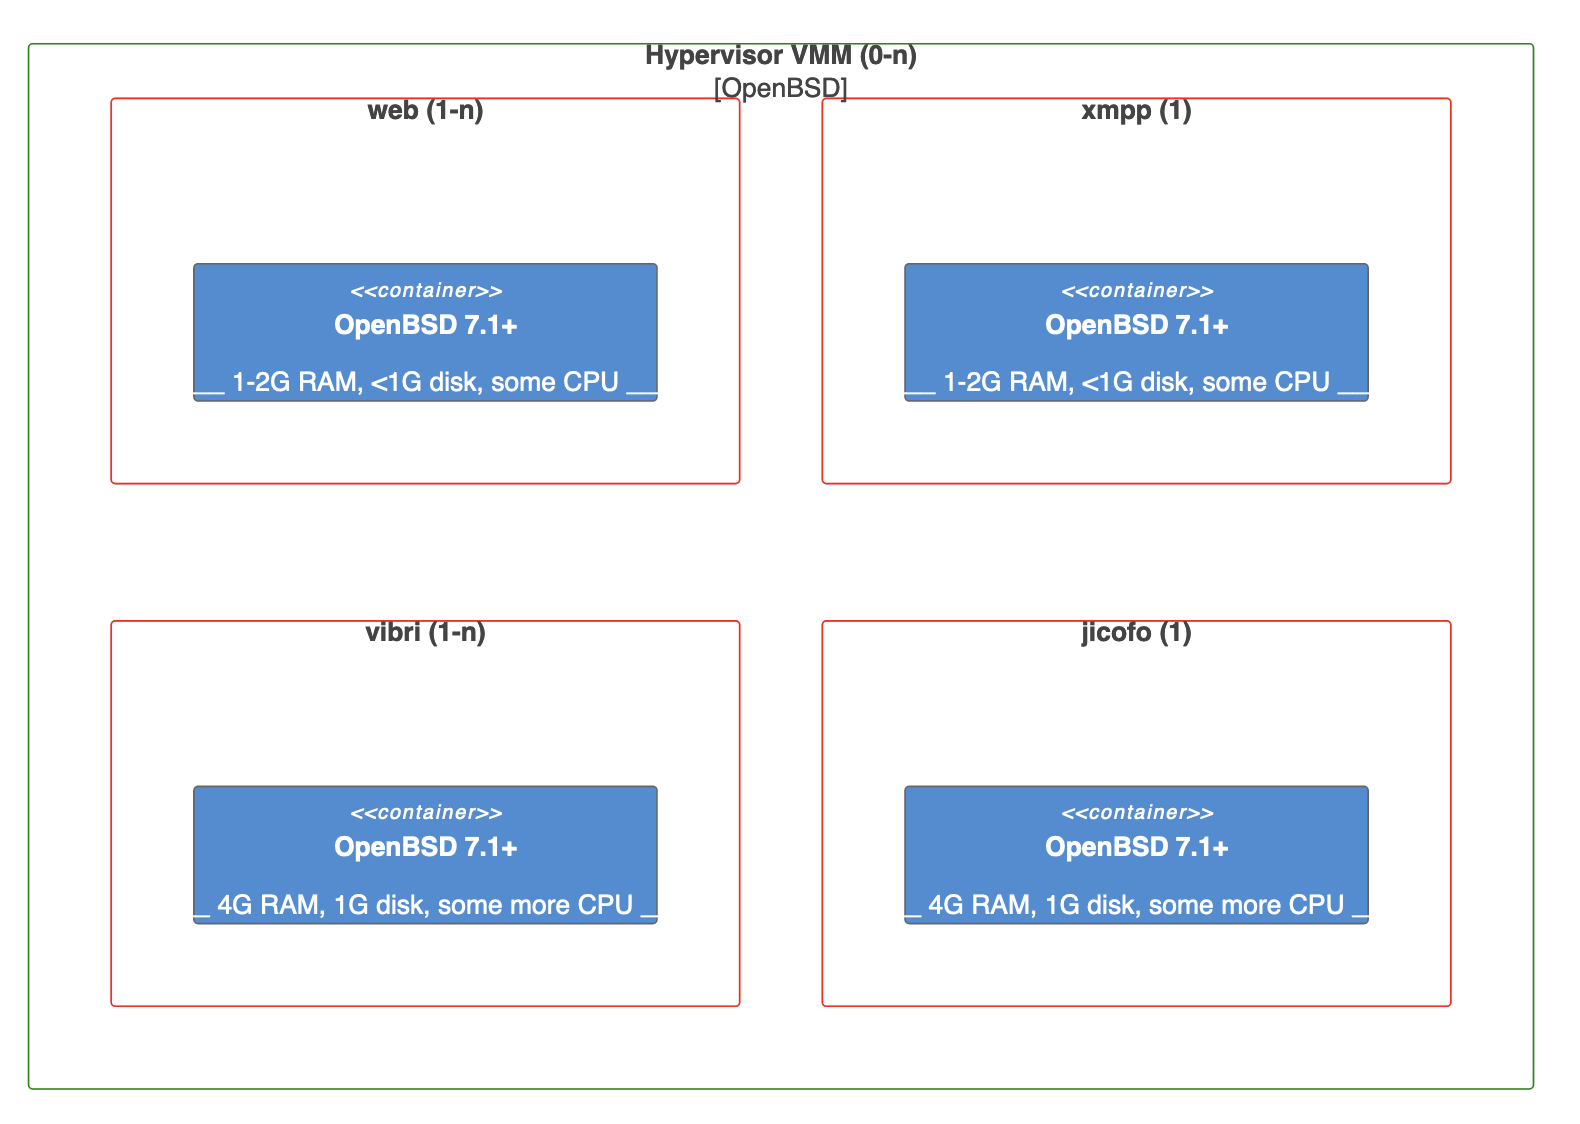
\includegraphics[width=16cm]{img/arch-openbsd.png}
    \caption{\textsf{OpenBSD VMM architecture}}
\end{figure*}
\section{Communications}
Communication between the components and the logical `publication` + `subscription` in Jitsi
is as follows (needed in `pf.conf` later on) (see Figure 2+3).
\begin{figure*}
    \centering
    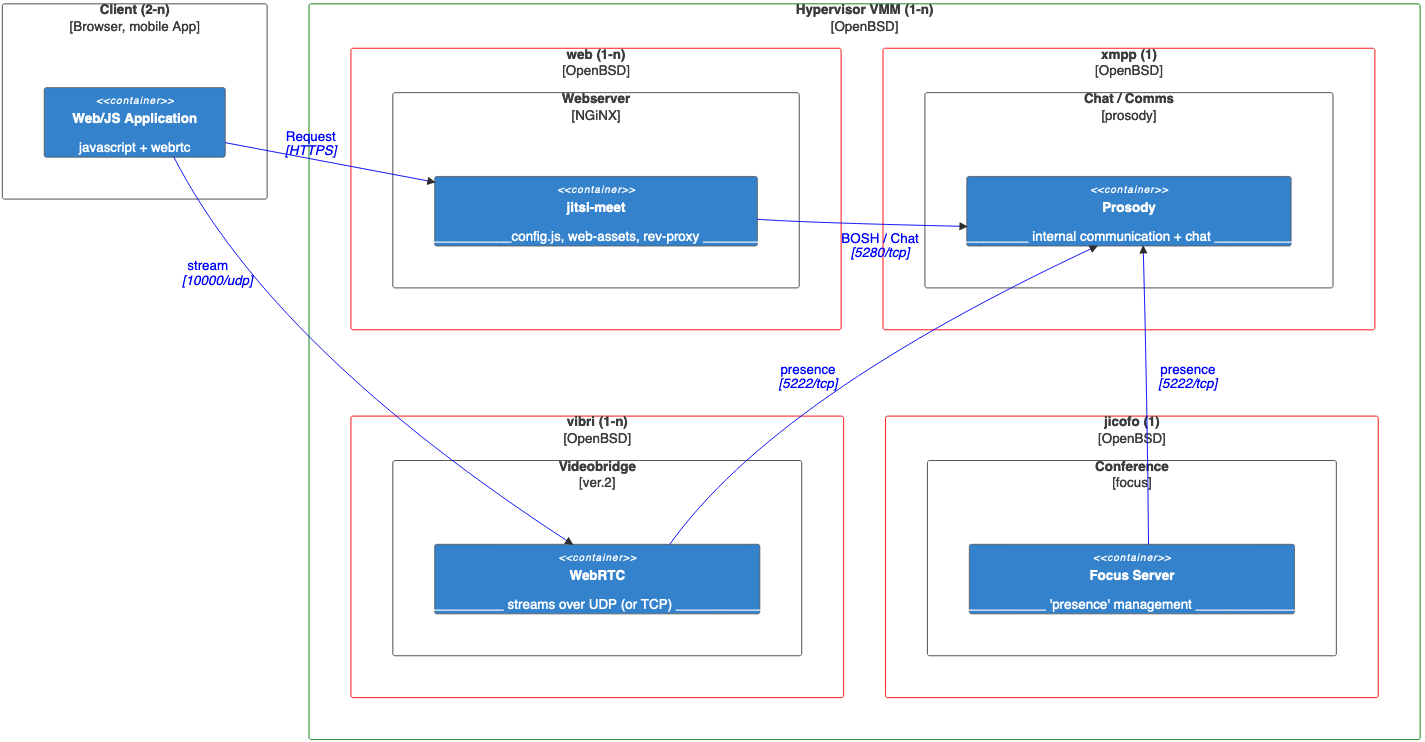
\includegraphics[width=16cm]{img/arch-tcp.png}
    \caption{\textsf{OpenBSD VMM architecture}}
\end{figure*}
\begin{figure*}
    \centering
    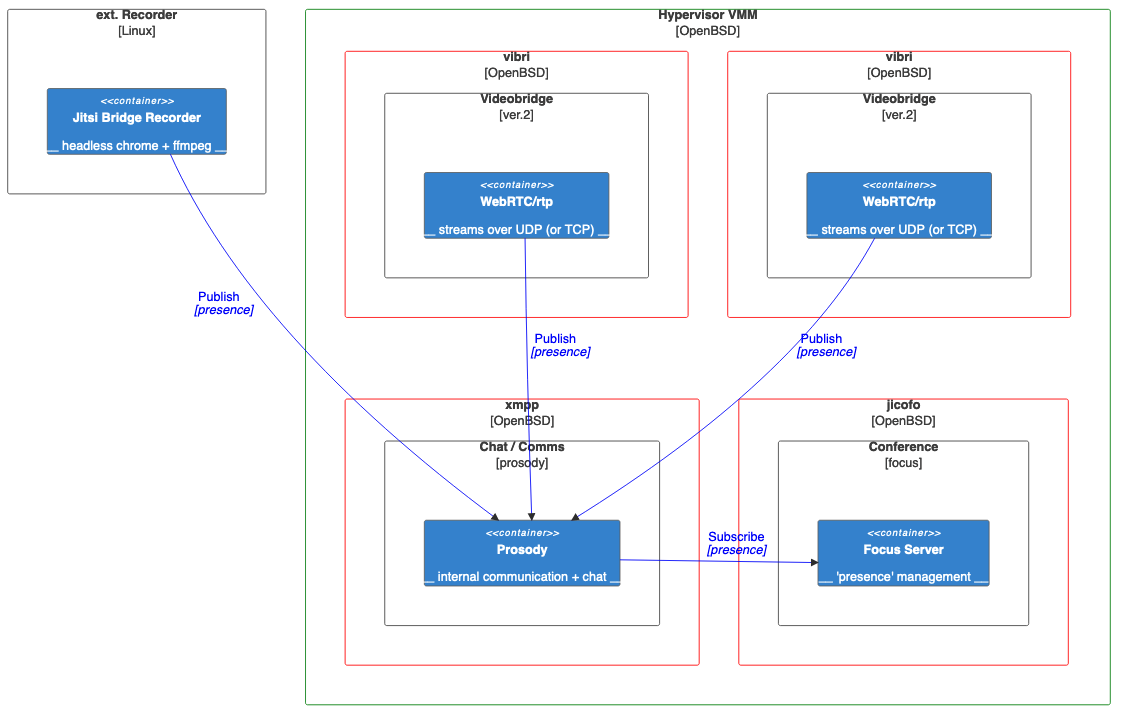
\includegraphics[width=16cm]{img/arch-pubsub.png}
    \caption{\textsf{OpenBSD VMM architecture}}
\end{figure*}

\section{Installation}
The installation is structered in the following steps:
\begin{itemize}
\item create VM images
\item construct /etc/vm.conf
\item add hosts / DNS
\item `nginx`: install, config, certs
\item `prosody`: pkg install, config, certs, users
\item `jicofo`: pkg install, config
\item `jvb`: pkg install, config
\end{itemize}

\subsection{VM setup}
To create an VM image being used in the following setup:
\begin{minted}{bash}
rcctl enable vmd
rcctl start vmd
mkdir /home/vmm; cd /home/vmm
vmctl create -s 5G web.qcow2
ftp https://cdn.openbsd.org/pub/OpenBSD\
/7.1/amd64/install71.iso
vmctl start -m 2G -L -i 1 -r install71.iso\
-d /home/vmm/web.qcow2 web
vmctl console web

## run the (I)nstaller, default options.
## only one 'a' slice on (w)hole disk
## halt -p (so new sshd_keys per VM)

vmctl stop web
for vm in xmpp jicofo jvb ; do
cp web.qcow2 ${vm}.qcow2; done
echo 'net.inet.ip.forwarding=1' >> \\
/etc/sysctl.conf
\end{minted}

The VM definitions in `/etc/vm.conf` are as follows. The "instance" keyword tells `vmctl`
to use "web"'s configuration as a template and only adapt changes like "disk"
or "memory" to it.

\begin{minted}{bash}
vm "web" {
  enable
  memory 2G
  disk "/home/vmm/web.qcow2" format qcow2
  local interface { up }
}
vm "web" instance "xmpp" {
  disk "/home/vmm/xmpp.qcow2" format qcow2
}
vm "web" instance "jicofo" {
  memory 4G
  disk "/home/vmm/jicofo.qcow2" format qcow2
}
vm "web" instance "jvb" {
  memory 4G
  disk "/home/vmm/jvb.qcow2" format qcow2
}
\end{minted}

\subsection{DNS + /etc/hosts}
DNS is only ONE A-RR for "jts.fips.de"; but local `/etc/hosts` for jicofo (or split DNS).

The following `/etc/hosts` needs to be on each VM and on the VMM host.
Use these names in `/etc/myname`, too.

\begin{minted}{bash}
100.64.1.3    web
100.64.2.3    xmpp jts.fips.de
100.64.3.3    jicofo
100.64.4.3    jvb
\end{minted}

\section{Firewalling}
On each VM the following `pf.conf` is for good (admin) measure:

\begin{minted}{bash}
block return log
pass out quick on egress proto { tcp udp }
  to any port { 123 53 80 443 }
pass in quick on egress proto tcp
  from $admin to port 22
\end{minted}

\subsection{VMM}
Assumption is that all traffic comes via the VMM external IP-address (on egress) here:

\begin{minted}{bash}
pass in on egress proto tcp to any
  port { 80 443 } rdr-to web
pass in on egress proto udp to any
  port { 10000 } rdr-to jvb
pass in proto tcp from { jvb jicofo }
  to xmpp port 5222 # native
pass in proto tcp from web to xmpp
  port 5280 # http/BOSH
pass in on egress proto tcp to any
  port 5280 rdr-to xmpp # debug
# DNS
vms={ web xmpp jicofo jvb }
pass in proto { udp tcp } from $vms
  to any port domain rdr-to $resolver
\end{minted}

\subsection{web/nginx}
The webserver needs the basic ports and for the proxy connection to BOSH an outgoing
to 5280/tcp.

\begin{minted}{bash}
pass in quick on egress proto tcp
  to self port { 80 443 }
pass out quick on egress proto tcp
  to xmpp port 5280
\end{minted}

\subsection{prosody}
The XMPP "native" only used from jicofo and jvb. The BOSH like as above and if need be
the dedicated auth via 5347/tcp (not covered here).

\begin{minted}{bash}
pass in proto tcp from { jicofo jvb }
  to self port { 5222 }
pass in proto tcp from web
  to self port 5280
pass in proto tcp from { $admin }
  to self port { 5280 5347} # debug
\end{minted}

\subsection{jicofo}
Jicofo talks to prosody as above. The webclient connects to jicofo via 10000/udp. There
is an administrative connection possible to 8080/tcp to establish e.g. monitoring with
prometheus.
To scale out the 10000/udp can be changed and would make use of a port range e.g. 
"10000:10050" vertically or explicit "rdr-to"s in VMM for horizontally.

\begin{minted}{bash}
pass out quick on egress proto
  tcp to xmpp port { 5222 5280 }
pass in quick on egress proto
  udp to self port 10000
pass in quick on egress proto
  tcp from $monitor to self port 8080
\end{minted}

\subsection{videobridge}
The videobridge only needs to reach out to prosody. The monitoring exporter on 8888/tcp
seems to be broken (no values) as of this writing.
\begin{minted}{bash}
pass out quick on egress proto
  tcp to xmpp port 5222
pass in quick on egress proto
  tcp from $monitor to self port 8888
\end{minted}

\section{Prosody}
To install prosody some simple steps are enough.

\begin{minted}{bash}
pkg_add unzip--
pkg_add prosody
pkg_add jitsi-prosody-plugins
\end{minted}

The `jitsi-prosody-plugins` does contain two needed plugins and some more for use
cases not mentioned in this document. Need be is `mod_client_proxy` and `mod_roster_command`.
The modules do not need further configuration in `prosody.cfg.lua`.
`client_proxy` gets loaded from the "Component" configuration.
For CLI use only is `roster_command`.

The configuration key bits in `/etc/prosody/prosody.cfg.lua` are:

\begin{minted}{bash}
http_interfaces = { "*", "::" }
VirtualHost "jts.fips.de"
    authentication = "anonymous";

    modules_enabled = { "bosh";
      "pubsub"; }
    c2s_require_encryption = false

VirtualHost "auth.jts.fips.de"
    admins = { "focus@auth.jts.fips.de",
     "jvb@auth.jts.fips.de" }

    ssl = { key =
     "/var/prosody/auth.jts.fips.de.key";
        certificate =
    "/var/prosody/auth.jts.fips.de.crt"; }

    authentication = "internal_hashed"

Component "conference.jts.fips.de" "muc"
Component "jvb.jts.fips.de"
    component_secret = "CHANGE_jvb"
Component "focus.jts.fips.de" "client_proxy"
    target_address =
      "focus@auth.jts.fips.de"
Component "internal.auth.jts.fips.de" "muc"
    muc_room_locking = false
    muc_room_default_public_jids = true
\end{minted}

The additional `FQDN` are prosody internal only and
do NOT need any DNS configuration (works like an
HTTP `Host` header).

It's possible that `jvb` follows the example of
`focus` to change authentication from shared secret
to a user (`target_address`).

\subsection{Users}
The connection for `jvb` uses a shared secret as shown in the previous configuration.
The further users in use here:

\begin{minted}{bash}
rcctl enable prosody
rcctl start prosody
prosodyctl register focus \
  auth.jts.fips.de CHANGE_FOCUS
prosodyctl mod_roster_command \
  subscribe focus.jts.fips.de \
  focus@auth.jts.fips.de
\end{minted}

\subsection{TLS}
Besides WebRTC demanding the use of `https` between browser and server side, we shall
encrypt all internal traffic, too. For the prosody connections:

\begin{minted}{bash}
prosodyctl cert generate \
  auth.jts.fips.de
# fill in the shown `openssl req` dialog

cd /var/prosody
yes | /usr/local/jdk-11/bin/keytool
  -import -alias prosody -file \
  auth.jts.fips.de.crt -keystore \
  jicofo-key.store -storepass jitsicool

cp jicofo-key.store jvb-key.store
# copy to VM jicofo and jvb accordingly
\end{minted}

`keytool` comes with the JDK package and this task can also be done on jicofo or jvb VM
- or copy over the resulting store-files to the jicofo/jvb VM respectivly.

Do NOT change JDK's `lib/security/cacerts` - any later upgrade of JDK
would overwrite the changed keystore and result in a loss of comms.

\section{nginx}
To install nginx and the jitsi web elements (javascript, images, ..) only two packages
are needed:

\begin{minted}{bash}
pkg_add nginx
pkg_add jitsi-meet
\end{minted}

A TLS setup is mandatory for brwoser/jvb or it will refuse to let you
use the camera and microphone.
Using Let's Encrypt with `acme-client(1)` for the TLS setup is easily possible and included
in `./testing-config/nginx.conf` (see "Availability" section).

\subsection{web}
The configuration for nginx is pretty straight forward:
\begin{minted}{bash}
server_name  jts.fips.de;
root         /var/www/jitsi-meet;

ssi on;
ssi_types application/x-javascript
  application/javascript;

location ~ ^/(libs|css|static|images|
  fonts|lang|sounds|
  connection_optimization)/(.*)$ {
  add_header
    'Access-Control-Allow-Origin' '*';
  alias /var/www/jitsi-meet/$1/$2; }

location /external_api.js { alias
  /var/www/jitsi-meet/libs/external_api.min.js; }

location = /http-bind {   # BOSH
  proxy_pass      http://xmpp:5280/http-bind;
  proxy_set_header X-Forwarded-For
    $remote_addr;
  proxy_set_header Host $http_host; }

location ~ ^/([a-zA-Z0-9=\?]+)$ {
  rewrite ^/(.*)$ / break; }
\end{minted}

If using Let's Encrypt, put the `.well-known` location first after `ssi` configuration block.

\subsection{jitsi-web}
The configuration for the webclient goes to `/var/www/jitsi-meet/config.js`:
\begin{minted}{bash}
var config = {
  hosts: {
    domain: 'jts.fips.de',
    muc: 'conference.jts.fips.de'
  },
  bosh: '//jts.fips.de/http-bind',
  useTurnUdp: false,
  	enableWelcomePage: true,
  prejoinConfig: {
    enabled: true,
    hideExtraJoinButtons:
      ['no-audio', 'by-phone'] },
  p2p: {
    stunServers: [
    { urls:
     'stun:meet-jit-si-turnrelay.jitsi.net:443'
    } ] }
}
\end{minted}
The use of TURN servers depend on NAT environment(s), most often it is needed (esp. p2p).

\section{jicofo}
The installation is one package and the configuration is split into two files plus
adaptions of the infra/systems configuration.

\subsection{JVM / startup}

\begin{minted}{bash}
pkg_add jicofo
cat << EOF > /etc/jicofo/jicofo.in.sh
JICOFO_CONF=/etc/jicofo/jicofo.conf
JICOFO_LOG_CONFIG=\
 /usr/local/share/\
 jicofo/lib/logging.properties
JICOFO_TRUSTSTORE=\
 /etc/ssl/jicofo-key.store
JICOFO_TRUSTSTORE_PASSWORD=jitsicool
JICOFO_MAXMEM=3G
JICOFO_DHKEYSIZE=2048
JAVA_SYS_PROPS=""
EOF
\end{minted}

jicofo-key.store is generated from prosody certificate, see prosody in section `VIII/B`.
One can enable an XMPP-packet-debug-log in logging.properties if need be.

\subsection{Parameters}
The main configuration for jicofo is `/etc/jicofo/jicofo.conf`:

\begin{minted}{bash}
jicofo { bridge {
  brewery-jid =
    "JvbBrewery@internal.auth.jts.fips.de"
  xmpp-connection-name = Client }
  sctp { enabled = false }
  xmpp {
    client {
      port = 5222
      domain = "auth.jts.fips.de"
      username = "focus"
      password = "CHANGE_FOCUS"
      use-tls = true
    }
    // trusted service domains.
    //  Logged in -> advance to bridges
    trusted-domains =
      [ "auth.jts.fips.de" ]
  }
}
\end{minted}

For proper startup and reachability it's needed to add ``jicofo_flags="--host=jts.fips.de"''
to `/etc/rc.conf.local`. This needs to be present in `/etc/hosts` or in (split) DNS and the
resolved IP address must point to the VM's local address! Since this is used as a matching
string for "virtual host" one cannot use an IP address here!

For proper logging add this to syslog configuration and then jicofo can be started
\begin{minted}{bash}
cat <<EOF >> /etc/syslog.conf
!jicofo
*.*     /var/log/jicofo
EOF
rcctl enable jicofo
rcctl start jicofo
\end{minted}

\section{videobridge}
The installation is one package and the configuration is split into two files plus
adaptions of the infra/systems configuration.

Installing `jitsi-srtp` is optional, but the speedup in encryption of WebRTC is substantial.
There's no additional configuration needed, if present JVB will load the native library just by
standard means (`ld.so(1)`).

\subsection{JVM / startup}

\begin{minted}{bash}
pkg_add jitsi-videobridge
pkg_add jitsi-srtp
cat << EOF > /etc/jicofo/jvb.in.sh
JVB_CONF=/etc/jvb/jvb.conf
JVB_LOG_CONFIG=\
 /usr/local/share/jvb/lib/logging.properties
JVB_TRUSTSTORE=/etc/ssl/jvb-key.store
JVB_TRUSTSTORE_PASSWORD=jitsicool
JVB_MAXMEM=3G
JVB_DHKEYSIZE=2048
JVB_GC_TYPE=G1GC
JAVA_SYS_PROPS=""

#/etc/jvb/sip-communicator.properties
JVB_SC_HOME_LOCATION='/etc'
JVB_SC_HOME_NAME='jvb'
EOF
\end{minted}
jvb-key.store is generated from prosody certificate as for jicofo. Can be same file
as /etc/jicofo/jicofo-key.store if both are on one VM.
\subsection{Parameters}
The main configuration file is `/etc/jvb/jvb.conf` as referenced above.
\begin{minted}{bash}
videobridge { apis {
  xmpp-client {
   configs {
    ourprosody {
     hostname = "xmpp"
     domain =
      "auth.jts.fips.de" // realm
     username = "jvb"
     password = "CHANGE_jvb"
     muc_jids =
      "JvbBrewery@internal.auth.jts.fips.de"
     muc_nickname = "jvb-foo"
     disable_certificate_verification =
      true
    } } } }
  sctp { enabled = false } // n/a on OpenBSD
  ice { tcp {
    enabled = false
    port = 443
   } udp {
    port = 10000
   }
  }
}
\end{minted}
The `JvbBrewery` part is a fixed string and cannot be replaced!

A third party library needs its own configuration file in `/etc/jvb/sip-communicator.properties`
as referenced in `jvb.in.sh`. The following must be written in three lines and are just
split up due to format reasons.
\begin{minted}{bash}
org.ice4j.ice.harvest.\
 NAT_HARVESTER_LOCAL_ADDRESS=100.64.4.3
org.ice4j.ice.harvest.\
 NAT_HARVESTER_PUBLIC_ADDRESS=87.253.170.146
org.ice4j.ice.harvest.\
 DISABLE_AWS_HARVESTER=true
\end{minted}
The LOCAL is the VMs internal address, the PUBLIC must be the one "presented" to the
outside world (e.g. nat-to on egress).

JVB does not need any `rc.conf` settings, but add this for logging and startup:
\begin{minted}{bash}
cat <<EOF >> /etc/syslog.conf
!jvb
*.*     /var/log/jvb
EOF
rcctl enable jvb
rcctl start jvb
\end{minted}

\section{Pitfalls / Hints}
There are some typical pitfalls that should be avoided eventually.

\subsection{OpenBSD}
\begin{itemize}
\item `rc.conf`: using IP address instead of hostname/FQDN
\item startup ordering: nginx, prosody, jicofo, jvb -- or wait times increase (pubsub)
\end{itemize}

\subsection{Jitsi}
Jitsi can have some more subtle ones and some are just advisable.
\begin{itemize}
\item xmpp: host vs. virtualhost vs. domain
\item DNS: one and only one (or mess up xmpp fallback)
\item not disabling sctp (jvb AND jicofo)
\item (hidden) version bumps ("no longer component!")
\item jicofo has an XMPP-packetlogger (see `logging.properties`)
\item patience, be really patient (at initial start)
\item always check the `,` in config.js (JSON after all..)
\end{itemize}

\section{Status}
It works! Most of the packages have landed in 7.2 already:
\begin{itemize}
\item `net/jitsi/meet`
\item `net/jitsi/jicofo`
\item `net/jitsi/videobridge`
\item `net/jitsi/srtp`
\item `net/jitsi/prosody-plugins`
\end{itemize}

A `meta` package to bundle all of the above is still in development/review.

\section{Outlook}
The jitsi component `jibri` for recording and/or streaming conferences can only run
on Linux for now. Main work would be needed to realize that in an Alpine or NixOS VM or
going the long way to get "chromedriver" running on OpenBSD.

Another component might be `jigasi` for SIP/POTS, but unsure about demand and feasability.

\section{Acknowledgments}
I want to make a shoutout to `Jitsi` and `OpenBSD` of course. A sincere "THANK YOU" to
Aisha Tammy spending lots of effort on making the packages and get them upstream.

My employer to be thanked as well allowing so many hours working on this project.


\section{Availability}
This paper, presentation slides and other directly related resources can be found on github:
\url{https://github.com/double-p/presentations/AsiaBSDCon/2022/}


\begin{thebibliography}{00}
\bibitem{b1} OpenBSD project \url{https://www.openbsd.org/}
\bibitem{b2} Jitsi \url{https://github.com/jitsi/}
\bibitem{b3} sysfive.com GmbH \url{https://www.sysfive.com/}
\end{thebibliography}

\section{Logfiles}
Some typical logfiles pointing to "known" errors:
\begin{minted}{bash}
# wrong/missing keystore [in prosody logfile]:
Sep 16 14:35:58 c2s60a86b47480  info
  Client connected
Sep 16 14:35:58 c2s60a86b47480  info
  Client disconnected: sslv3 alert certificate unknown

# wrong password [in prosody logfile]:
Sep 16 14:36:20 c2s60b1aced0c0  info
  Stream encrypted (TLSv1.3 with TLS_AES_256_GCM_SHA384)
Sep 16 14:36:21 c2s60b1aced0c0  info
  Client disconnected: connection closed

# all good [in prosody logfile]:
Sep 16 14:37:00 c2s60a5b549900  info
  Stream encrypted (TLSv1.3 with TLS_AES_256_GCM_SHA384)
Sep 16 14:37:01 c2s60a5b549900  info
  Authenticated as focus@auth.jts.fips.de

# on cannot use a jvb before this log [in jicofo logging]:
Jicofo 2022-09-16 14:45:24.260 INFO: [35]
 [type=bridge brewery=jvbbrewery]
 BaseBrewery.addInstance#341: Added brewery
 instance: jvbbrewery@internal.auth.jts.fips.de/jvb

# JVB loading SRTP lib (only active connections)
INFO: [71] JitsiOpenSslProvider.<clinit>#52:
 jitsisrtp successfully loaded for OpenSSL 1.1
\end{minted}
\end{document}
